\section{System Details}
\subsection{Architecture of System}
\begin{frame}{Architecture of DSL}
\begin{figure}[H]
  \centering
    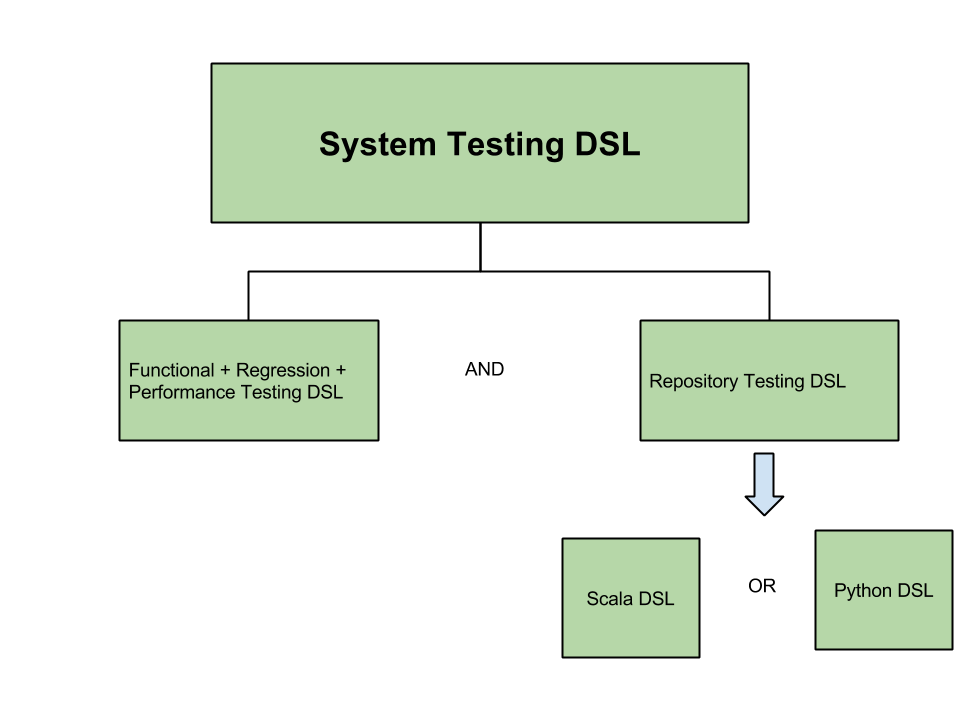
\includegraphics[width=250px]{figures/architecture.png}
  \caption{Architecture of System Testing DSL}
\end{figure}
\end{frame}

\begin{frame}{Composition of DSLs}
\begin{figure}[H]
  \centering
    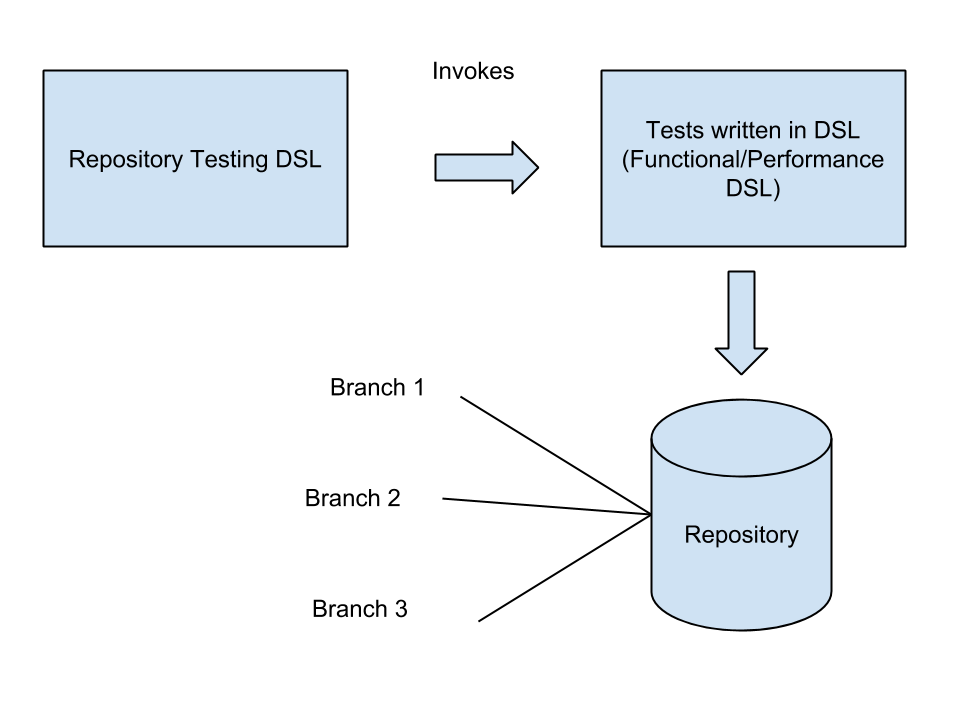
\includegraphics[width=230px]{figures/repo_test_diagram.png}
    \caption{Composition Repository Testing and Functional/Performance Testing DSL}
\end{figure}
\end{frame}

\subsection{Features}
\begin{frame}{Features}
\begin{itemize}
\item Regression Testing
\item Functional Testing
\item Performance Testing
\item Repository Testing
\end{itemize}
\end{frame}

\begin{frame}{Regression Testing}
\begin{figure}[H]
  \centering
    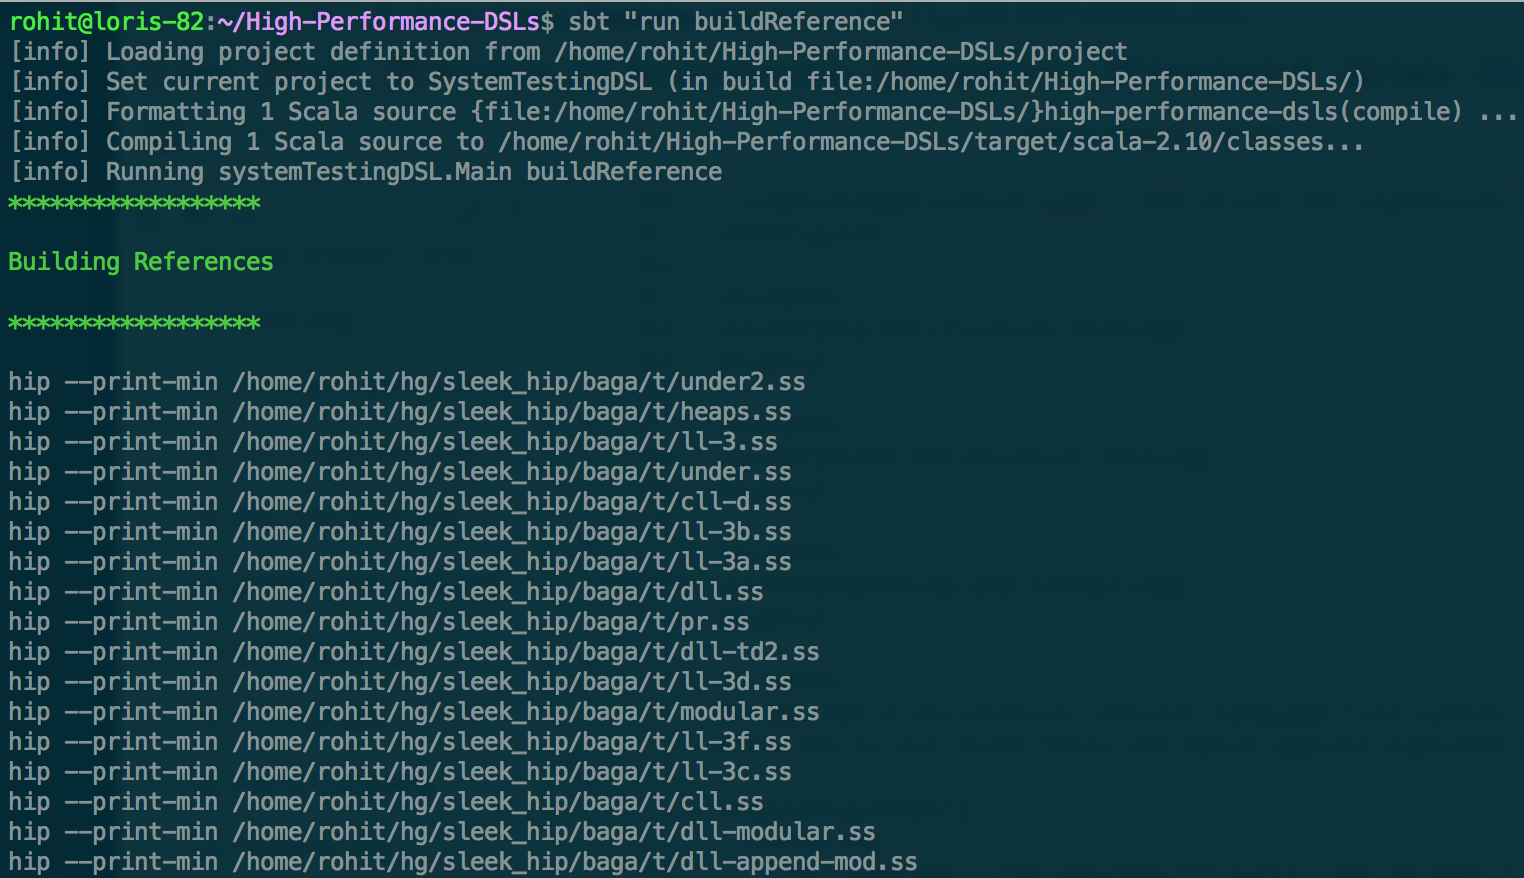
\includegraphics[width=300px]{figures/building_reference.png}
  \caption{Building References for Regression Testing}
\end{figure}
\end{frame}

\begin{frame}{Regression Testing}
\begin{block}{Running Regression Tests}
3 primary options provided - \textbf{buildReference, runReference and overrideReference}. The first one creates a repository of reference results for specified tests. The second option runs a set of tests against the stored references. The last option is for selectively rebuilding reference results.
\end{block}
\end{frame}

\begin{frame}{Functional Testing - Sleek}
\begin{figure}[H]
  \centering
    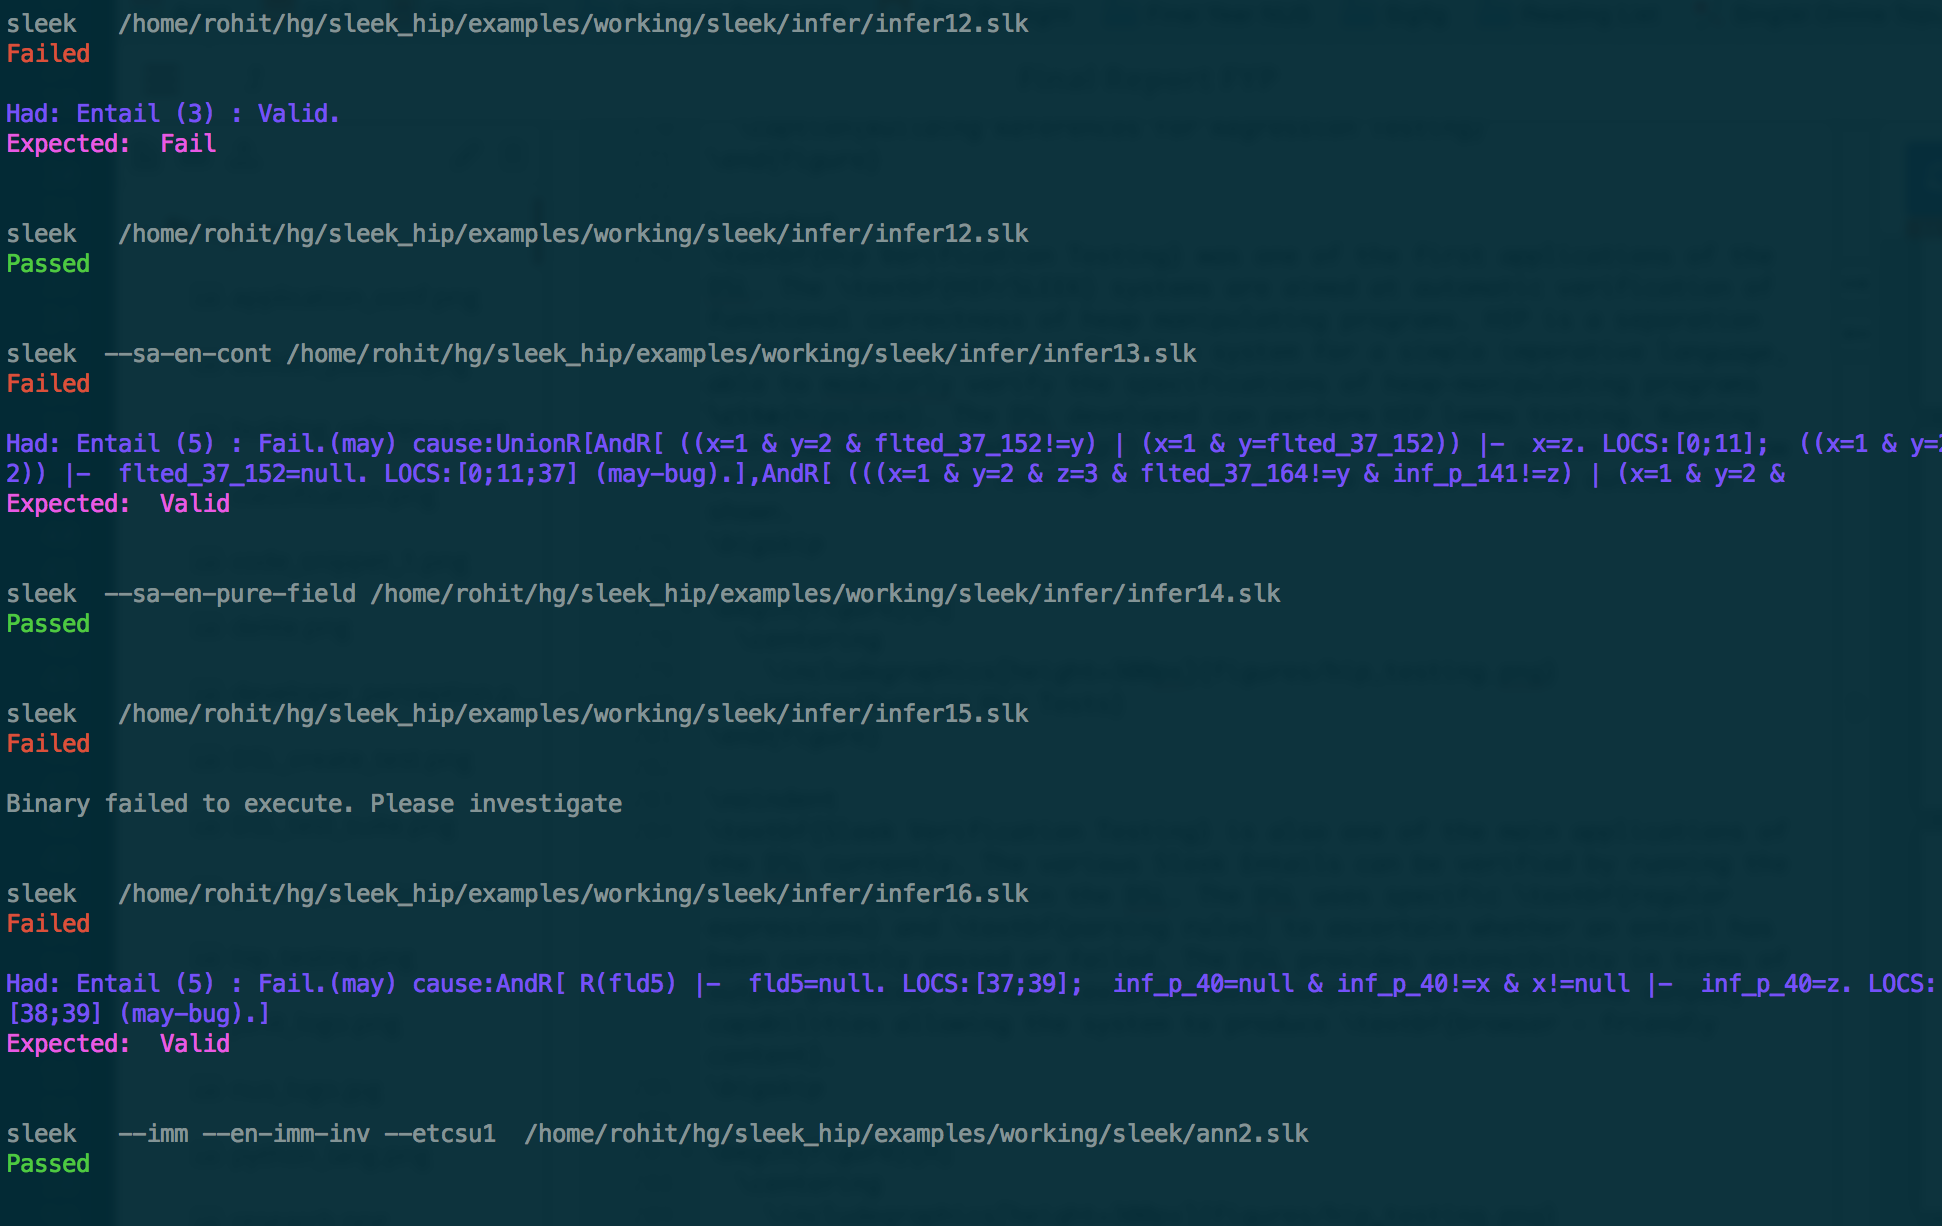
\includegraphics[width=300px]{figures/sleek_testing.png}
  \caption{Running Sleek Tests Console Output}
\end{figure}
\end{frame}

\begin{frame}{Functional Testing - Sleek}
\begin{figure}[H]
  \centering
    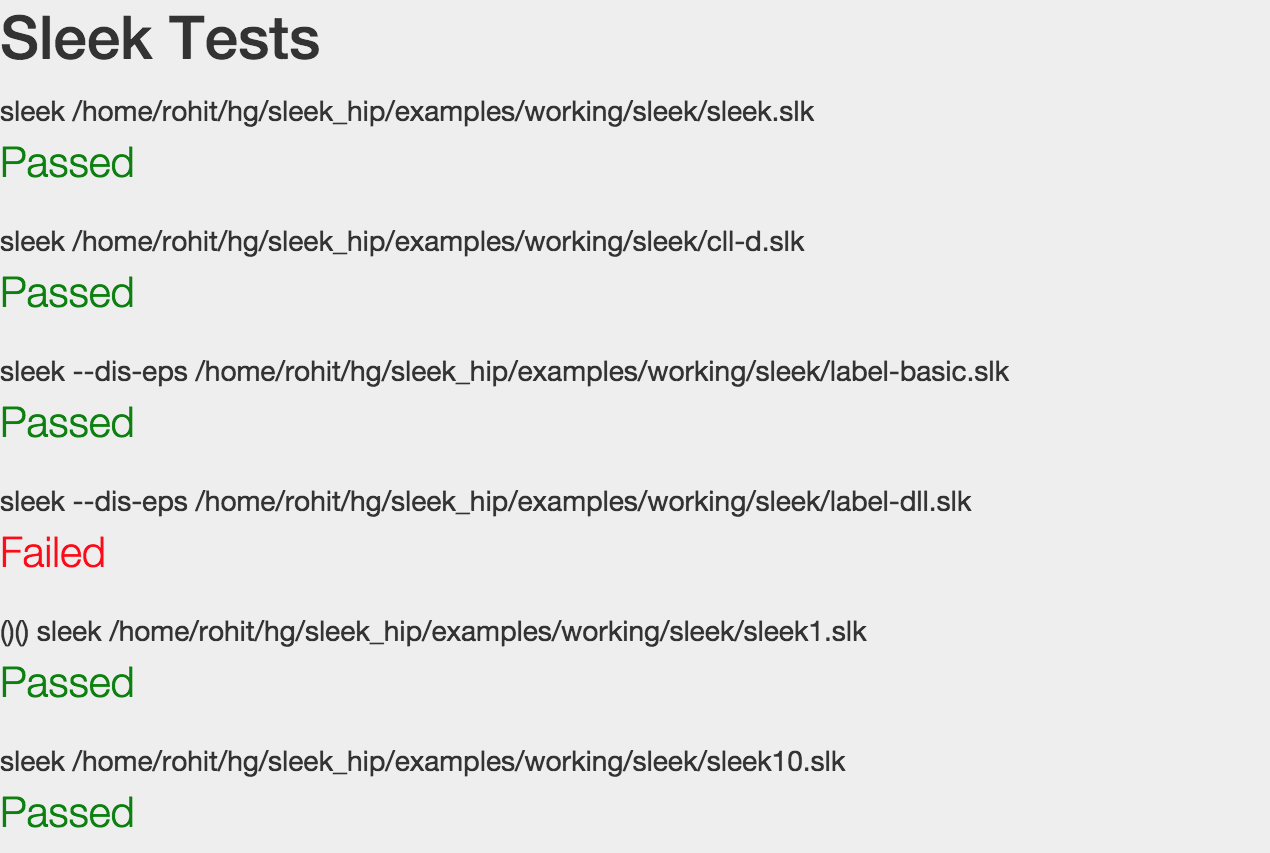
\includegraphics[width=280px]{figures/web_output_1.png}
  \caption{Running Sleek Tests HTML Output}
\end{figure}
\end{frame}

\begin{frame}{Performance Testing}
\begin{figure}[H]
  \centering
    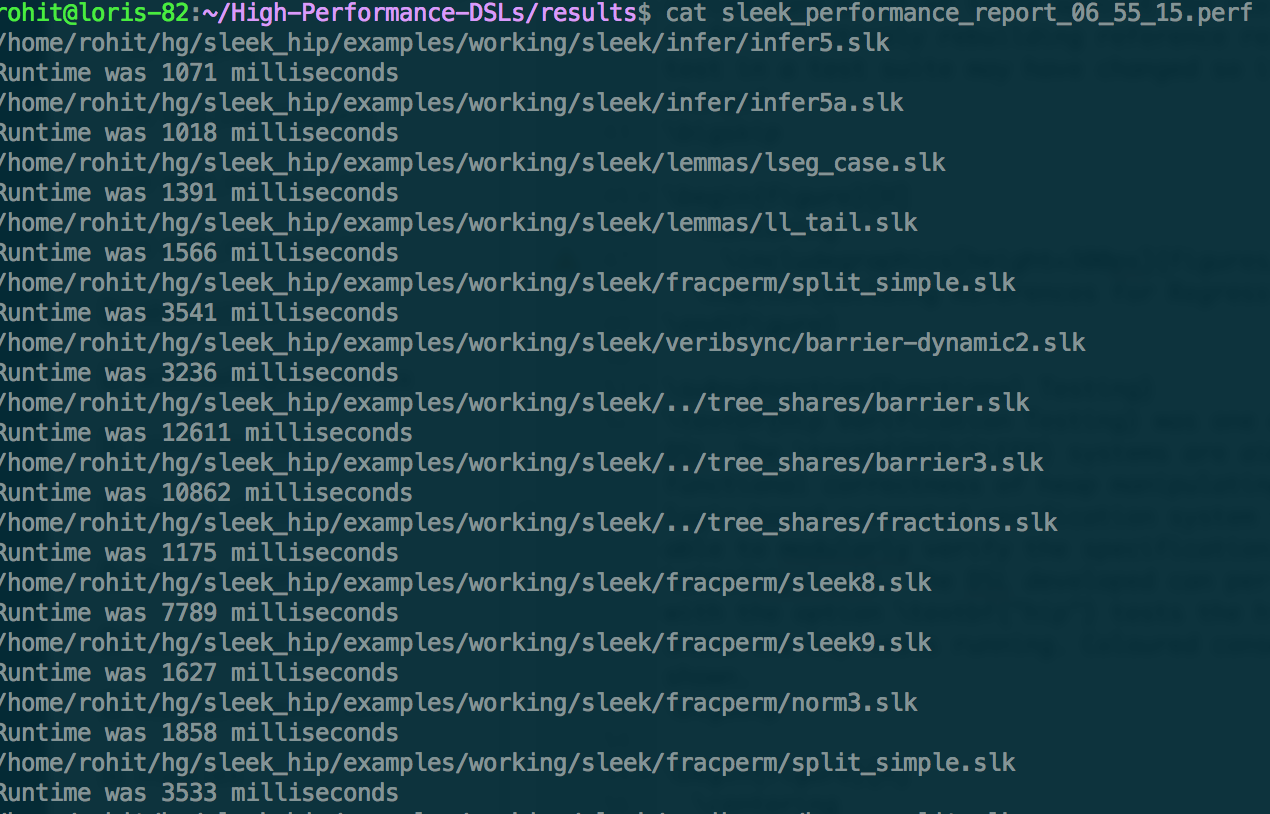
\includegraphics[width=300px]{figures/performance_testing.png}
  \caption{Performance Report for Sleek Tests}
\end{figure}
\end{frame}

\begin{frame}{Repository Testing}
\begin{figure}[H]
  \centering
    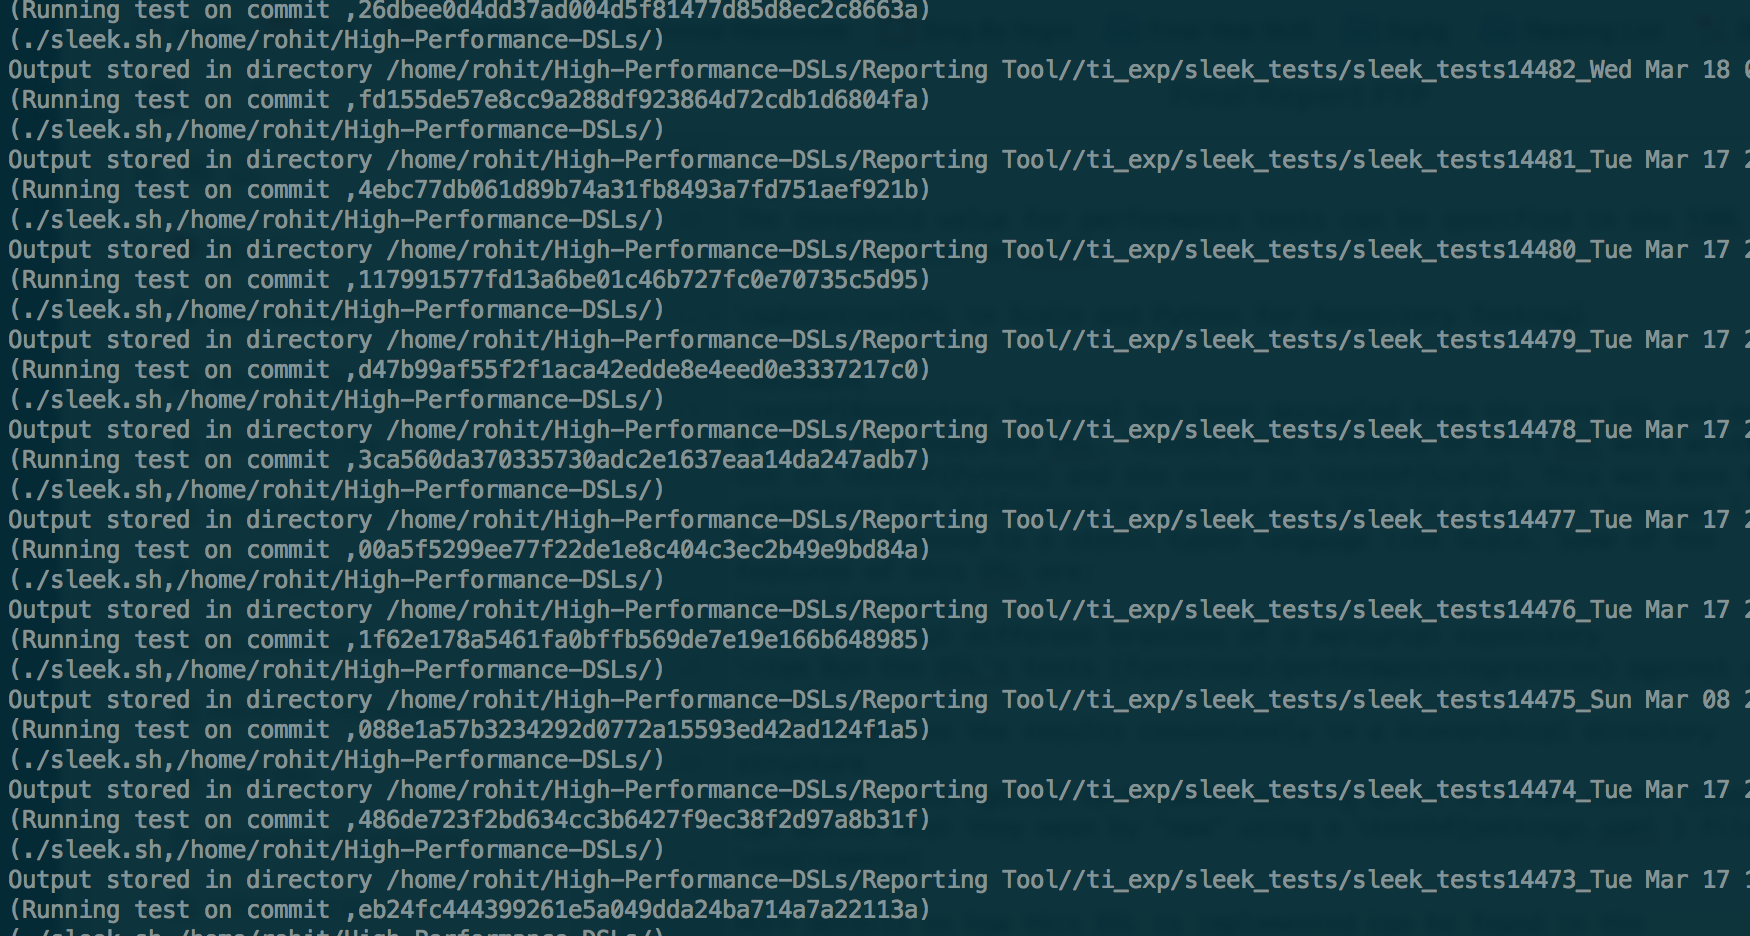
\includegraphics[width=300px]{figures/repo_testing.png}
  \caption{Repository level tests being run on the HIP/SLEEK code base}
\end{figure}
\end{frame}


\begin{frame}{Test Statistics}
\begin{figure}[H]
  \centering
    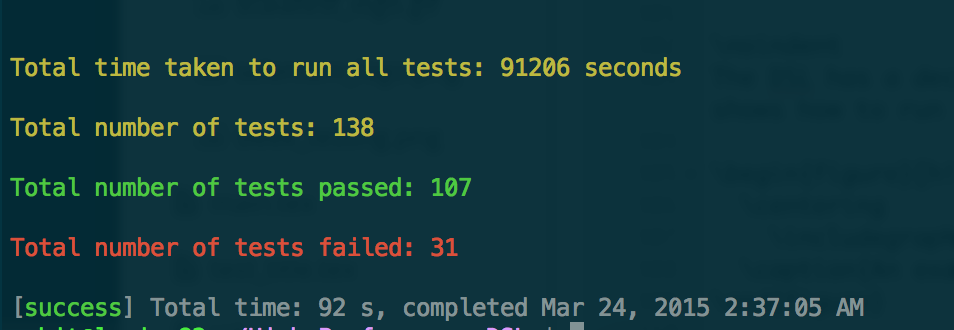
\includegraphics[width=300px]{figures/test_statistics.png}
  \caption{Test statistics at the end of every test Console Output}
\end{figure}
\end{frame}

\begin{frame}{Test Statistics}
\begin{figure}[H]
  \centering
    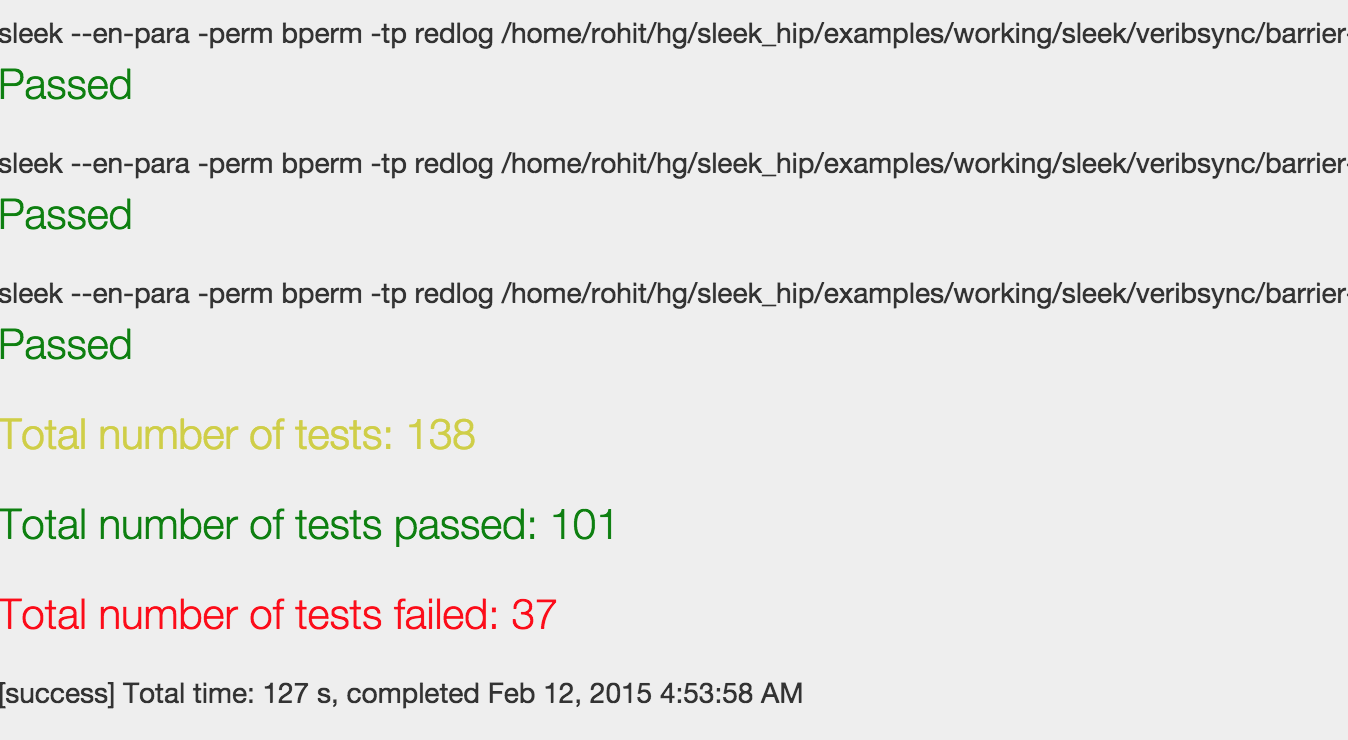
\includegraphics[width=300px]{figures/web_output_2.png}
  \caption{Test statistics at the end of every test HTML Output}
\end{figure}
\end{frame}

\begin{frame}{Test Statistics}
\begin{figure}[H]
  \centering
    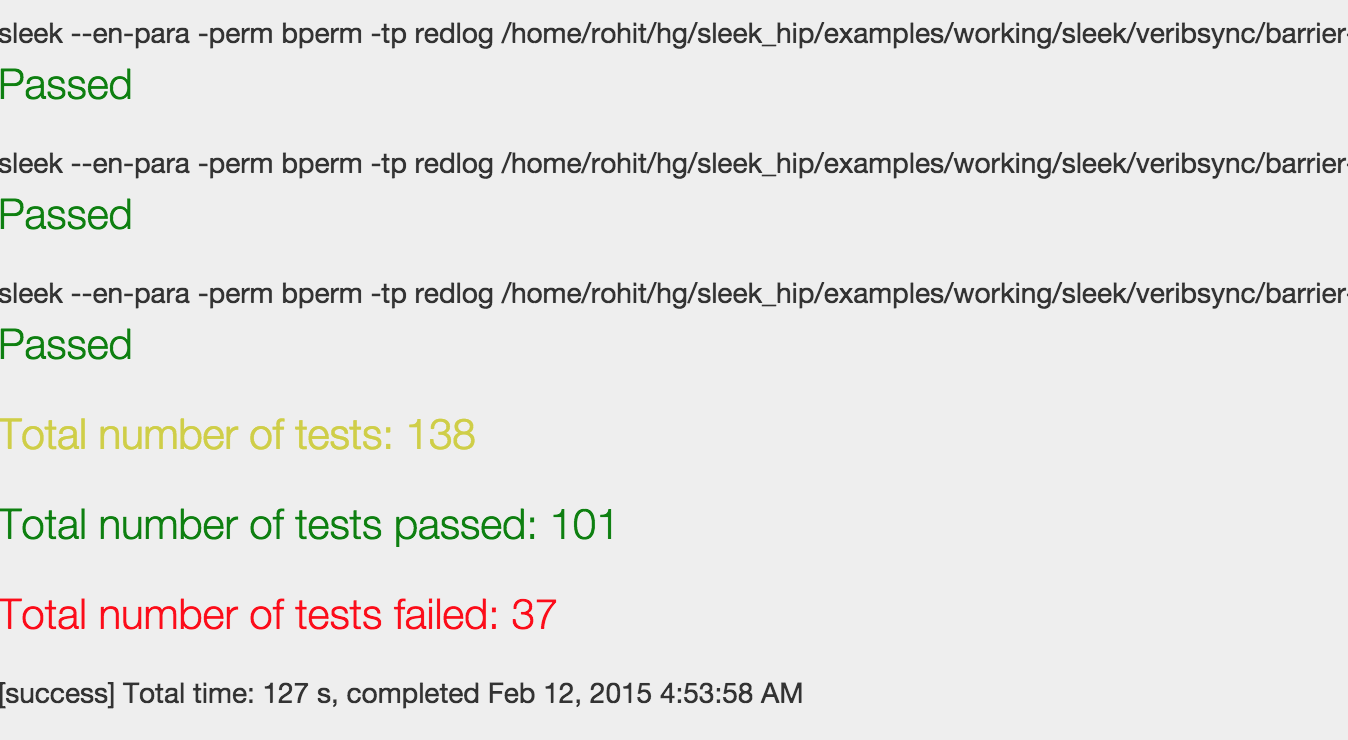
\includegraphics[width=300px]{figures/web_output_2.png}
  \caption{Test statistics at the end of every test HTML Output}
\end{figure}
\end{frame}

\begin{frame}

Demo

\end{frame}